% Created 2022-01-31 Mon 11:18
% Intended LaTeX compiler: pdflatex
\documentclass[presentation,aspectratio=169]{beamer}
\usepackage[utf8]{inputenc}
\usepackage[T1]{fontenc}
\usepackage{graphicx}
\usepackage{grffile}
\usepackage{longtable}
\usepackage{wrapfig}
\usepackage{rotating}
\usepackage[normalem]{ulem}
\usepackage{amsmath}
\usepackage{textcomp}
\usepackage{amssymb}
\usepackage{capt-of}
\usepackage{hyperref}
\usepackage{khpreamble}
\usepackage{amssymb}
\usepgfplotslibrary{groupplots}
\newcommand*{\shift}{\ensuremath{\operatorname{q}}}
\usetheme{default}
\author{Kjartan Halvorsen}
\date{\today}
\title{Cinemática - Representación de posición y orientación}
\hypersetup{
 pdfauthor={Kjartan Halvorsen},
 pdftitle={Cinemática - Representación de posición y orientación},
 pdfkeywords={},
 pdfsubject={},
 pdfcreator={Emacs 26.3 (Org mode 9.4.6)}, 
 pdflang={English}}
\begin{document}

\maketitle

\section{Intro}
\label{sec:org513471b}
\begin{frame}[label={sec:org376904c}]{Definiciones}
\begin{center}
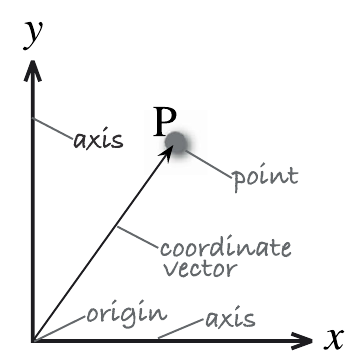
\includegraphics[height=0.5\textheight]{../figures/Corke-fig2.1.a.png}

\footnotesize Peter Corke \emph{Robotics, vision and control}
\end{center}
\end{frame}


\begin{frame}[label={sec:orgc1c60fc}]{Uso de sistemas de referencia en robótica}
\begin{center}
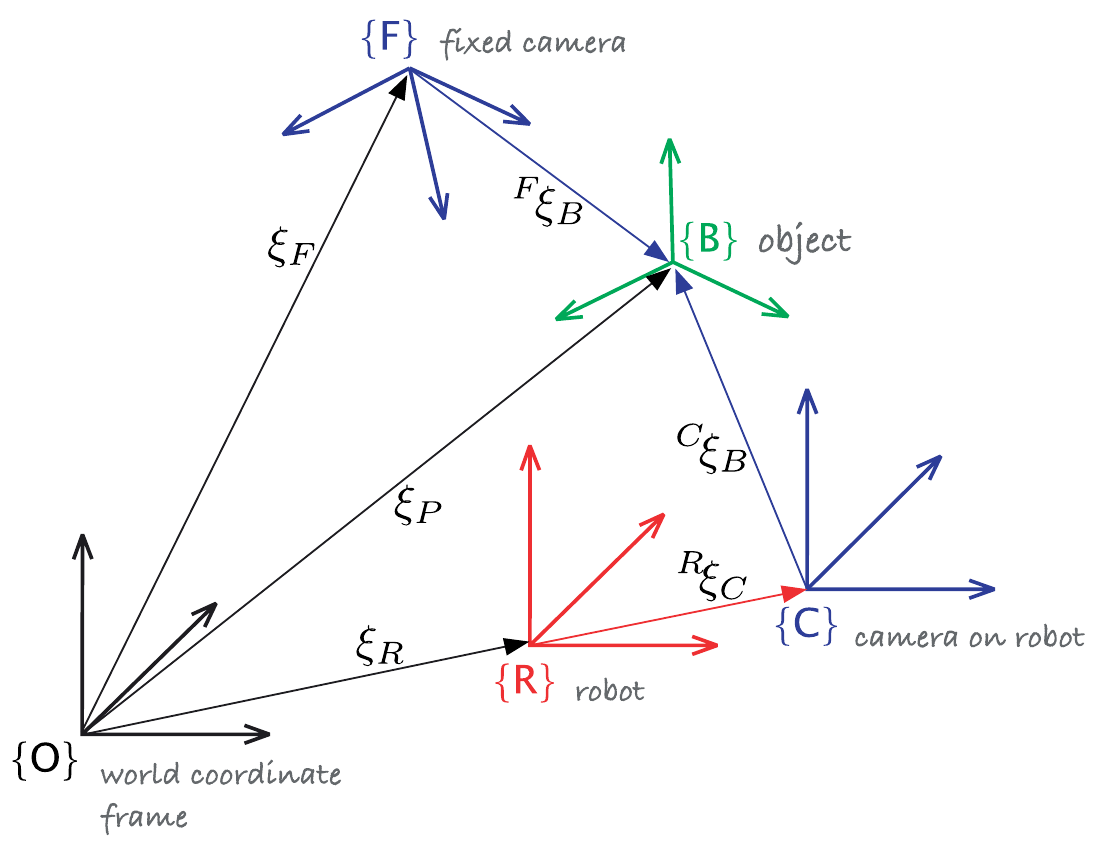
\includegraphics[height=0.5\textheight]{../figures/Corke-fig2.4.png}

\footnotesize Peter Corke \emph{Robotics, vision and control}
\end{center}
\end{frame}

\section{Pose en 2D}
\label{sec:org6f888b3}

\begin{frame}[label={sec:orga3bfcfd}]{Pose en 2D}
\begin{center}
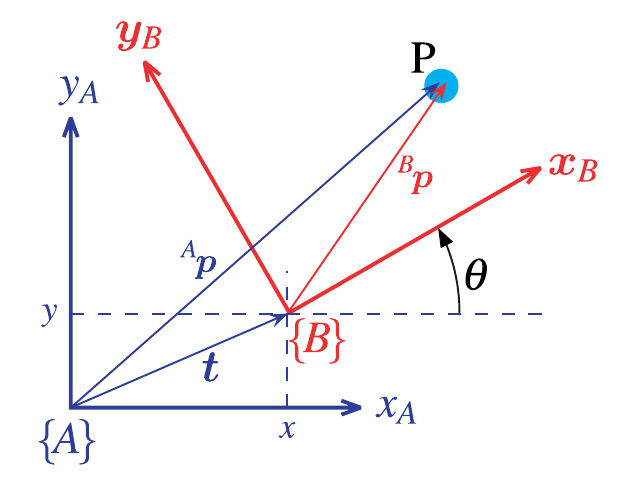
\includegraphics[height=0.5\textheight]{../figures/Corke-fig2.6.png}

\footnotesize Peter Corke \emph{Robotics, vision and control}
\end{center}
\end{frame}

\begin{frame}[label={sec:org5279996}]{Ejemplo}
\end{frame}


\begin{frame}[label={sec:org4562096}]{Ejercicio}
\end{frame}

\begin{frame}[label={sec:org5a851ac}]{Programar}
\end{frame}


\section{Pose en 3D}
\label{sec:org2afbba4}

\begin{frame}[label={sec:org96ac22c}]{Rotación en 3D}
\begin{center}
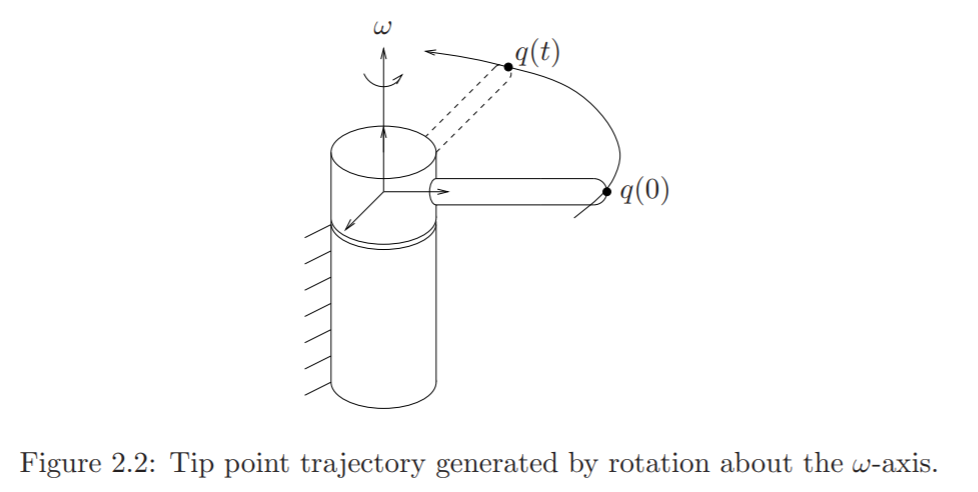
\includegraphics[height=0.5\textheight]{../figures/MLS-fig2.2.png}

\footnotesize Murray, Li and Sastry \emph{A mathematical introduction to robotic manipulation}
\end{center}
\end{frame}

\begin{frame}[label={sec:org91921d2}]{Mapa exponencial}
\end{frame}


\begin{frame}[label={sec:org1826315}]{Pose en 3D}
\end{frame}

\begin{frame}[label={sec:org5d0efb5}]{Coordenadas homogéneas}
\end{frame}
\end{document}